\documentclass[11pt,a4paper]{article}
\usepackage[margin=2cm]{geometry}
\usepackage{booktabs,graphicx,array,xcolor}
\setlength{\parindent}{0pt}
\setlength{\parskip}{5pt}
\begin{document}

\begin{center}
{\Large\bfseries Cable simulation: which approach to adopt}\\[2pt]
{\normalsize A decision brief --- compatibility first}
\end{center}

\textbf{The question.} A cable must be simulated as part of a larger system.
Several methods reproduce its hanging shape to within a few centimetres of a real
cable, so raw accuracy is \emph{not} the deciding factor. What decides it is
\textbf{what each approach is compatible with} --- which existing stack it plugs
into with the least friction --- because the cable is one component of a much
bigger project.

\textbf{One thing to know about accuracy.} The method closest to the textbook
mathematics is the \emph{furthest} from the real cable, and vice-versa. This is
not a solver being wrong: the real cable is held with tape that fixes its angle,
which the ideal curve does not model. Every method here is behaving correctly;
they differ in \emph{which} real-world detail they capture. So choose on
integration, and treat all of them as accurate enough to a few centimetres.

\vspace{4pt}
\renewcommand{\arraystretch}{1.25}
\begin{tabular}{@{}p{3.1cm} c c p{7.9cm}@{}}
\toprule
\textbf{Approach} & \textbf{vs real} & \textbf{speed} & \textbf{Integrates with} \\
\midrule
\textbf{PhysX capsule chain} & 33~mm & 29~s & Drops straight into an Isaac Sim / Omniverse project: USD-native, works with Isaac Lab, the ROS 2 bridge, sensors, and collision against robots and the environment. Real-time. \\[2pt]
\multicolumn{4}{p{\dimexpr\linewidth-2\tabcolsep}}{\footnotesize\itshape Best when the cable must live in, and interact with, an Isaac Sim scene. Watch: rigid-capsule approximation; not differentiable.} \\
\midrule
\textbf{Newton cable (add\_rod)} & 75~mm & 13~s & Native to the Newton / Warp stack: differentiable (gradients for control, learning, system identification) and GPU-batched for large-scale training. Newton is the forward-looking successor in the Isaac roadmap. \\[2pt]
\multicolumn{4}{p{\dimexpr\linewidth-2\tabcolsep}}{\footnotesize\itshape Best when high-fidelity cable physics, differentiability, or GPU-batched learning are needed. Watch: newer, evolving API; heavier per-step cost.} \\
\midrule
\textbf{Warp XPBD rod} & 51~mm & 1~s & A single self-contained Warp component with no engine dependency: differentiable, portable, easy to embed in a custom pipeline. You own the modelling (stiffness, resolution, boundary conditions). \\[2pt]
\multicolumn{4}{p{\dimexpr\linewidth-2\tabcolsep}}{\footnotesize\itshape Best when a lightweight or differentiable rod is wanted without a full engine. Watch: bending stiffness and mesh resolution must be calibrated; crudest bending model.} \\
\midrule
\bottomrule
\end{tabular}

\begin{figure}[h]\centering
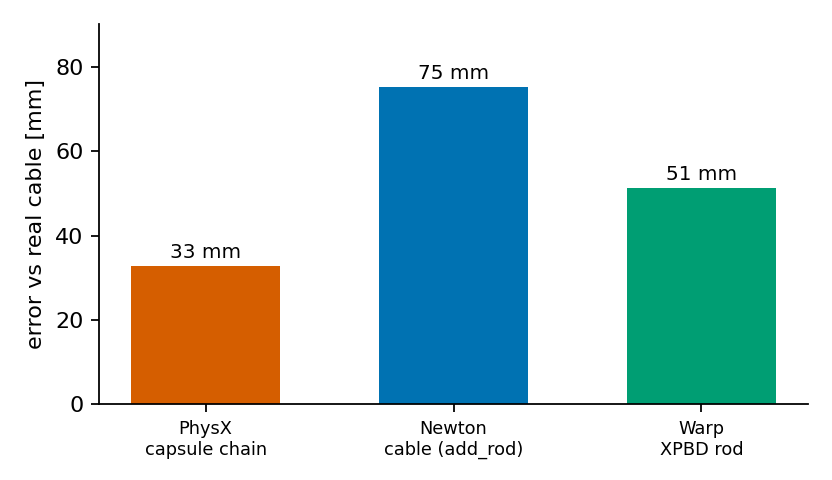
\includegraphics[width=0.66\linewidth]{accuracy.png}
\caption{Error against the photographed cable (lower is closer to reality).}\end{figure}

\begin{figure}[h]\centering
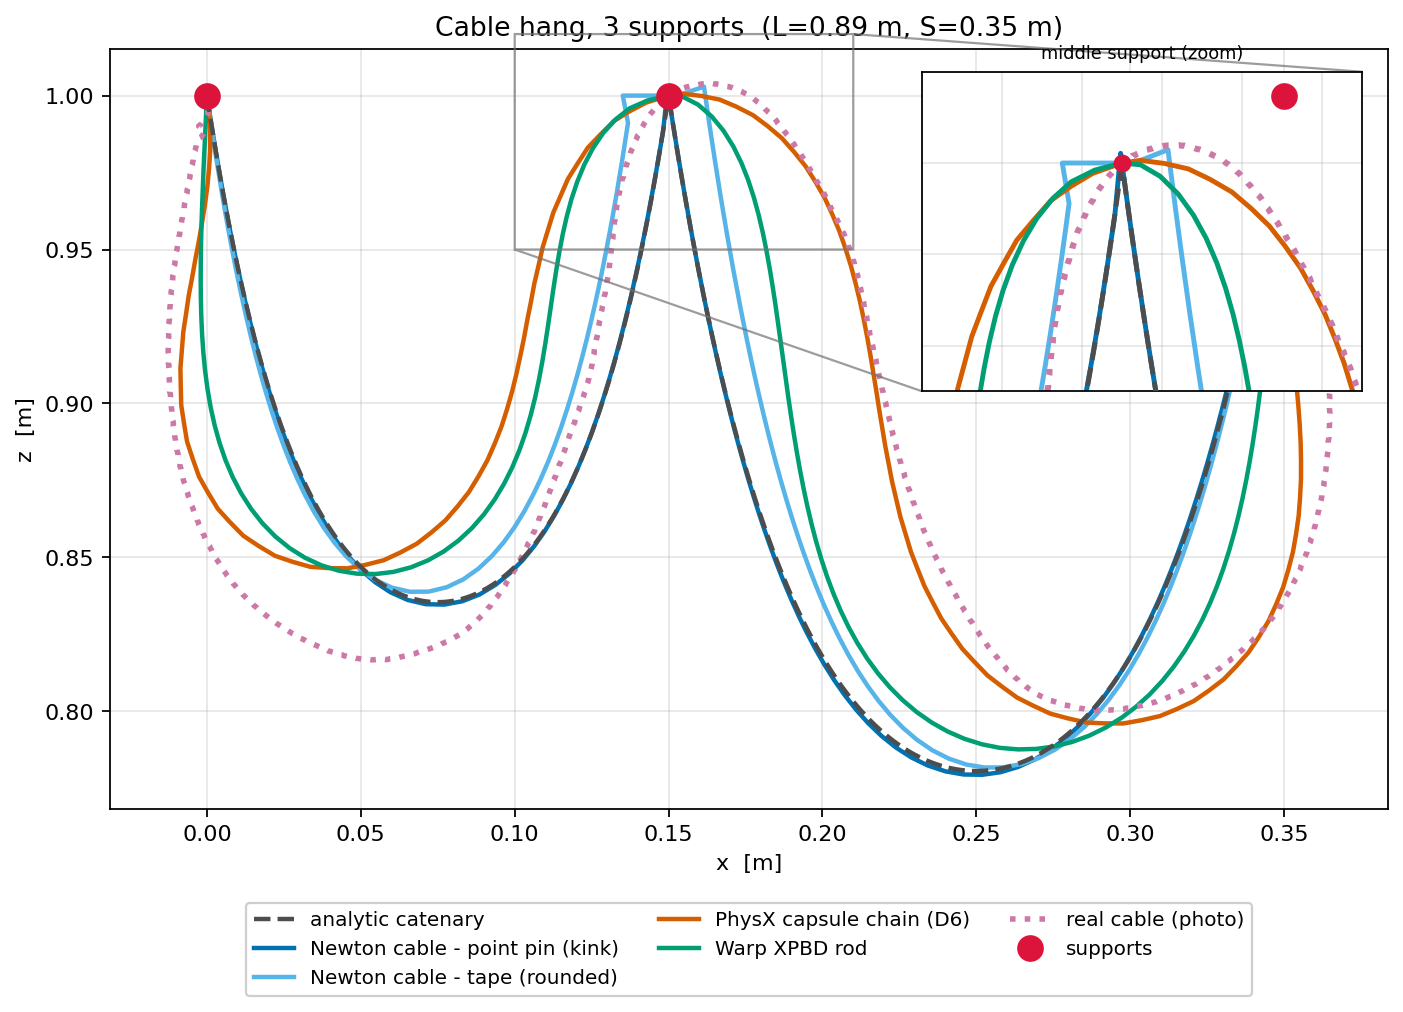
\includegraphics[width=0.86\linewidth]{overlay.png}
\caption{Every approach, the exact mathematics (dashed), and the real cable (dotted) on one axis. The methods bracket the real cable; the differences are boundary-condition modelling, not solver bugs.}\end{figure}

\textbf{Recommendation.}
\begin{itemize}
\setlength{\itemsep}{1pt}
\item If the wider project lives in \textbf{Isaac Sim / Omniverse} and the cable
      must interact with robots or the scene: \textbf{PhysX capsule chain}.
      Most compatible with what is already there, closest to the real cable, and
      real-time.
\item If the project needs \textbf{differentiability or GPU-batched learning},
      or is adopting \textbf{Newton}: \textbf{Newton cable}. Highest fidelity
      to the physics and future-facing, at a higher compute cost.
\item If a \textbf{lightweight, embeddable, engine-free} component is wanted:
      \textbf{Warp rod}. Fewest dependencies and differentiable, but you
      calibrate its stiffness and resolution.
\end{itemize}

\textbf{Ruled out on this build.} A Newton \emph{USD-engine} cable cannot be
fixed at both ends (an articulation must be a tree, a doubly-clamped cable is a
loop), and PhysX \emph{volumetric FEM} builds but its state cannot be read back.
Both fail with a clear diagnosis rather than silently. The three above are the
live options.

\end{document}
